% Created by tikzDevice version 0.12.3.1 on 2020-08-24 13:39:39
% !TEX encoding = UTF-8 Unicode
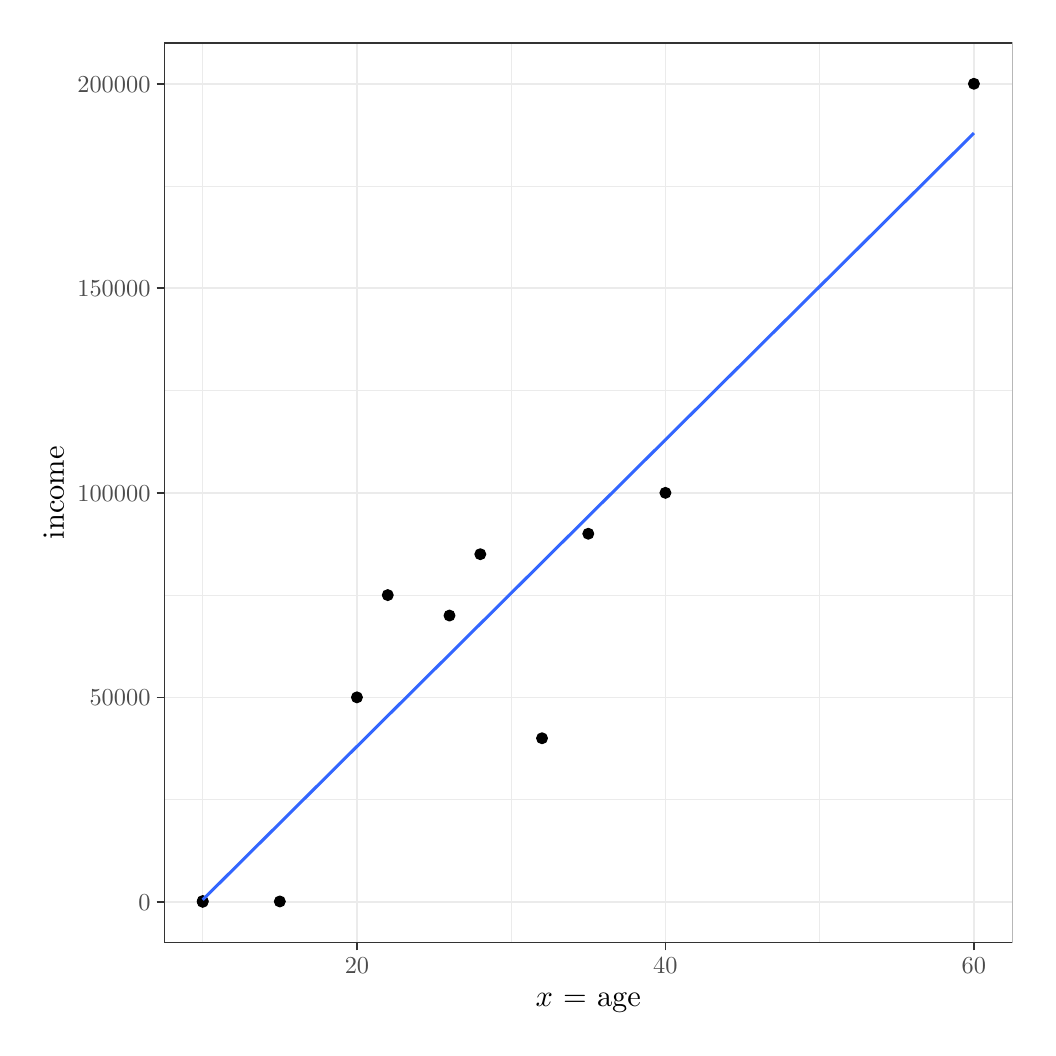
\begin{tikzpicture}[x=1pt,y=1pt]
\definecolor{fillColor}{RGB}{255,255,255}
\path[use as bounding box,fill=fillColor,fill opacity=0.00] (0,0) rectangle (361.35,361.35);
\begin{scope}
\path[clip] (  0.00,  0.00) rectangle (361.35,361.35);
\definecolor{drawColor}{RGB}{255,255,255}
\definecolor{fillColor}{RGB}{255,255,255}

\path[draw=drawColor,line width= 0.6pt,line join=round,line cap=round,fill=fillColor] (  0.00,  0.00) rectangle (361.35,361.35);
\end{scope}
\begin{scope}
\path[clip] ( 49.31, 30.69) rectangle (355.85,355.85);
\definecolor{fillColor}{RGB}{255,255,255}

\path[fill=fillColor] ( 49.31, 30.69) rectangle (355.85,355.85);
\definecolor{drawColor}{gray}{0.92}

\path[draw=drawColor,line width= 0.3pt,line join=round] ( 49.31, 82.41) --
	(355.85, 82.41);

\path[draw=drawColor,line width= 0.3pt,line join=round] ( 49.31,156.31) --
	(355.85,156.31);

\path[draw=drawColor,line width= 0.3pt,line join=round] ( 49.31,230.22) --
	(355.85,230.22);

\path[draw=drawColor,line width= 0.3pt,line join=round] ( 49.31,304.12) --
	(355.85,304.12);

\path[draw=drawColor,line width= 0.3pt,line join=round] ( 63.24, 30.69) --
	( 63.24,355.85);

\path[draw=drawColor,line width= 0.3pt,line join=round] (174.71, 30.69) --
	(174.71,355.85);

\path[draw=drawColor,line width= 0.3pt,line join=round] (286.18, 30.69) --
	(286.18,355.85);

\path[draw=drawColor,line width= 0.6pt,line join=round] ( 49.31, 45.46) --
	(355.85, 45.46);

\path[draw=drawColor,line width= 0.6pt,line join=round] ( 49.31,119.36) --
	(355.85,119.36);

\path[draw=drawColor,line width= 0.6pt,line join=round] ( 49.31,193.26) --
	(355.85,193.26);

\path[draw=drawColor,line width= 0.6pt,line join=round] ( 49.31,267.17) --
	(355.85,267.17);

\path[draw=drawColor,line width= 0.6pt,line join=round] ( 49.31,341.07) --
	(355.85,341.07);

\path[draw=drawColor,line width= 0.6pt,line join=round] (118.98, 30.69) --
	(118.98,355.85);

\path[draw=drawColor,line width= 0.6pt,line join=round] (230.45, 30.69) --
	(230.45,355.85);

\path[draw=drawColor,line width= 0.6pt,line join=round] (341.92, 30.69) --
	(341.92,355.85);
\definecolor{drawColor}{RGB}{0,0,0}
\definecolor{fillColor}{RGB}{0,0,0}

\path[draw=drawColor,line width= 0.4pt,line join=round,line cap=round,fill=fillColor] ( 63.24, 45.47) circle (  1.96);

\path[draw=drawColor,line width= 0.4pt,line join=round,line cap=round,fill=fillColor] ( 91.11, 45.61) circle (  1.96);

\path[draw=drawColor,line width= 0.4pt,line join=round,line cap=round,fill=fillColor] (230.45,193.26) circle (  1.96);

\path[draw=drawColor,line width= 0.4pt,line join=round,line cap=round,fill=fillColor] (118.98,119.36) circle (  1.96);

\path[draw=drawColor,line width= 0.4pt,line join=round,line cap=round,fill=fillColor] (130.12,156.31) circle (  1.96);

\path[draw=drawColor,line width= 0.4pt,line join=round,line cap=round,fill=fillColor] (341.92,341.07) circle (  1.96);

\path[draw=drawColor,line width= 0.4pt,line join=round,line cap=round,fill=fillColor] (202.58,178.48) circle (  1.96);

\path[draw=drawColor,line width= 0.4pt,line join=round,line cap=round,fill=fillColor] (185.86,104.58) circle (  1.96);

\path[draw=drawColor,line width= 0.4pt,line join=round,line cap=round,fill=fillColor] (163.56,171.09) circle (  1.96);

\path[draw=drawColor,line width= 0.4pt,line join=round,line cap=round,fill=fillColor] (152.42,148.92) circle (  1.96);

\path[draw=drawColor,line width= 0.4pt,line join=round,line cap=round,fill=fillColor] ( 63.24, 45.75) circle (  1.96);
\definecolor{drawColor}{RGB}{51,102,255}

\path[draw=drawColor,line width= 1.1pt,line join=round] ( 63.24, 46.20) --
	( 66.77, 49.71) --
	( 70.30, 53.22) --
	( 73.82, 56.72) --
	( 77.35, 60.23) --
	( 80.88, 63.74) --
	( 84.41, 67.24) --
	( 87.93, 70.75) --
	( 91.46, 74.26) --
	( 94.99, 77.76) --
	( 98.52, 81.27) --
	(102.04, 84.78) --
	(105.57, 88.29) --
	(109.10, 91.79) --
	(112.63, 95.30) --
	(116.15, 98.81) --
	(119.68,102.31) --
	(123.21,105.82) --
	(126.74,109.33) --
	(130.26,112.83) --
	(133.79,116.34) --
	(137.32,119.85) --
	(140.85,123.35) --
	(144.37,126.86) --
	(147.90,130.37) --
	(151.43,133.87) --
	(154.96,137.38) --
	(158.48,140.89) --
	(162.01,144.40) --
	(165.54,147.90) --
	(169.07,151.41) --
	(172.60,154.92) --
	(176.12,158.42) --
	(179.65,161.93) --
	(183.18,165.44) --
	(186.71,168.94) --
	(190.23,172.45) --
	(193.76,175.96) --
	(197.29,179.46) --
	(200.82,182.97) --
	(204.34,186.48) --
	(207.87,189.98) --
	(211.40,193.49) --
	(214.93,197.00) --
	(218.45,200.51) --
	(221.98,204.01) --
	(225.51,207.52) --
	(229.04,211.03) --
	(232.56,214.53) --
	(236.09,218.04) --
	(239.62,221.55) --
	(243.15,225.05) --
	(246.67,228.56) --
	(250.20,232.07) --
	(253.73,235.57) --
	(257.26,239.08) --
	(260.78,242.59) --
	(264.31,246.10) --
	(267.84,249.60) --
	(271.37,253.11) --
	(274.89,256.62) --
	(278.42,260.12) --
	(281.95,263.63) --
	(285.48,267.14) --
	(289.00,270.64) --
	(292.53,274.15) --
	(296.06,277.66) --
	(299.59,281.16) --
	(303.11,284.67) --
	(306.64,288.18) --
	(310.17,291.68) --
	(313.70,295.19) --
	(317.22,298.70) --
	(320.75,302.21) --
	(324.28,305.71) --
	(327.81,309.22) --
	(331.33,312.73) --
	(334.86,316.23) --
	(338.39,319.74) --
	(341.92,323.25);
\definecolor{drawColor}{gray}{0.20}

\path[draw=drawColor,line width= 0.6pt,line join=round,line cap=round] ( 49.31, 30.69) rectangle (355.85,355.85);
\end{scope}
\begin{scope}
\path[clip] (  0.00,  0.00) rectangle (361.35,361.35);
\definecolor{drawColor}{gray}{0.30}

\node[text=drawColor,anchor=base east,inner sep=0pt, outer sep=0pt, scale=  0.88] at ( 44.36, 42.43) {0};

\node[text=drawColor,anchor=base east,inner sep=0pt, outer sep=0pt, scale=  0.88] at ( 44.36,116.33) {50000};

\node[text=drawColor,anchor=base east,inner sep=0pt, outer sep=0pt, scale=  0.88] at ( 44.36,190.23) {100000};

\node[text=drawColor,anchor=base east,inner sep=0pt, outer sep=0pt, scale=  0.88] at ( 44.36,264.14) {150000};

\node[text=drawColor,anchor=base east,inner sep=0pt, outer sep=0pt, scale=  0.88] at ( 44.36,338.04) {200000};
\end{scope}
\begin{scope}
\path[clip] (  0.00,  0.00) rectangle (361.35,361.35);
\definecolor{drawColor}{gray}{0.20}

\path[draw=drawColor,line width= 0.6pt,line join=round] ( 46.56, 45.46) --
	( 49.31, 45.46);

\path[draw=drawColor,line width= 0.6pt,line join=round] ( 46.56,119.36) --
	( 49.31,119.36);

\path[draw=drawColor,line width= 0.6pt,line join=round] ( 46.56,193.26) --
	( 49.31,193.26);

\path[draw=drawColor,line width= 0.6pt,line join=round] ( 46.56,267.17) --
	( 49.31,267.17);

\path[draw=drawColor,line width= 0.6pt,line join=round] ( 46.56,341.07) --
	( 49.31,341.07);
\end{scope}
\begin{scope}
\path[clip] (  0.00,  0.00) rectangle (361.35,361.35);
\definecolor{drawColor}{gray}{0.20}

\path[draw=drawColor,line width= 0.6pt,line join=round] (118.98, 27.94) --
	(118.98, 30.69);

\path[draw=drawColor,line width= 0.6pt,line join=round] (230.45, 27.94) --
	(230.45, 30.69);

\path[draw=drawColor,line width= 0.6pt,line join=round] (341.92, 27.94) --
	(341.92, 30.69);
\end{scope}
\begin{scope}
\path[clip] (  0.00,  0.00) rectangle (361.35,361.35);
\definecolor{drawColor}{gray}{0.30}

\node[text=drawColor,anchor=base,inner sep=0pt, outer sep=0pt, scale=  0.88] at (118.98, 19.68) {20};

\node[text=drawColor,anchor=base,inner sep=0pt, outer sep=0pt, scale=  0.88] at (230.45, 19.68) {40};

\node[text=drawColor,anchor=base,inner sep=0pt, outer sep=0pt, scale=  0.88] at (341.92, 19.68) {60};
\end{scope}
\begin{scope}
\path[clip] (  0.00,  0.00) rectangle (361.35,361.35);
\definecolor{drawColor}{RGB}{0,0,0}

\node[text=drawColor,anchor=base,inner sep=0pt, outer sep=0pt, scale=  1.10] at (202.58,  7.64) {$x$ =  age};
\end{scope}
\begin{scope}
\path[clip] (  0.00,  0.00) rectangle (361.35,361.35);
\definecolor{drawColor}{RGB}{0,0,0}

\node[text=drawColor,rotate= 90.00,anchor=base,inner sep=0pt, outer sep=0pt, scale=  1.10] at ( 13.08,193.27) {income};
\end{scope}
\end{tikzpicture}
